\begin{figure}[htbp]
  \centering
  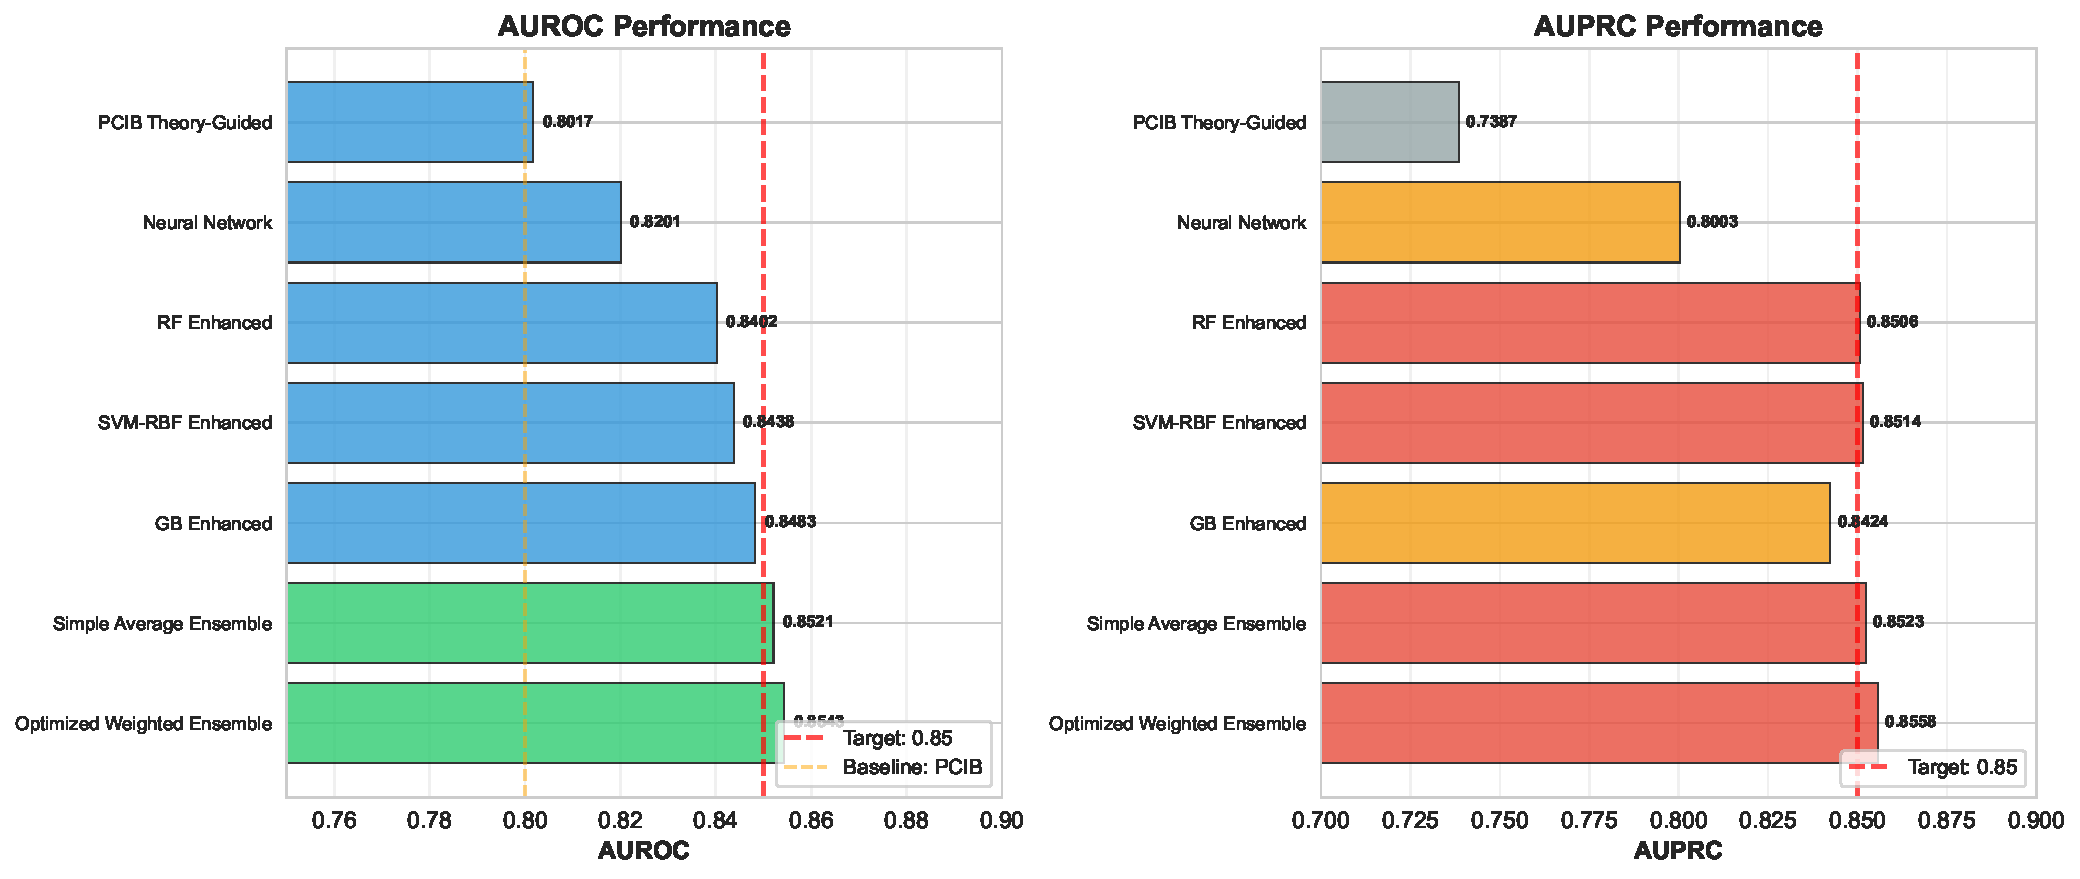
\includegraphics[width=\textwidth]{stacking_performance.pdf}
  \caption{Performance comparison of PCIB signal stacking approaches. Left: AUROC scores showing all methods exceed 0.80, with ensemble methods achieving 0.85+. Right: AUPRC scores demonstrating consistent improvements across metrics. The dashed lines indicate target (0.85) and baseline PCIB (0.80) performance levels.}
  \label{fig:stacking_comparison}
\end{figure}

\begin{figure}[htbp]
  \centering
  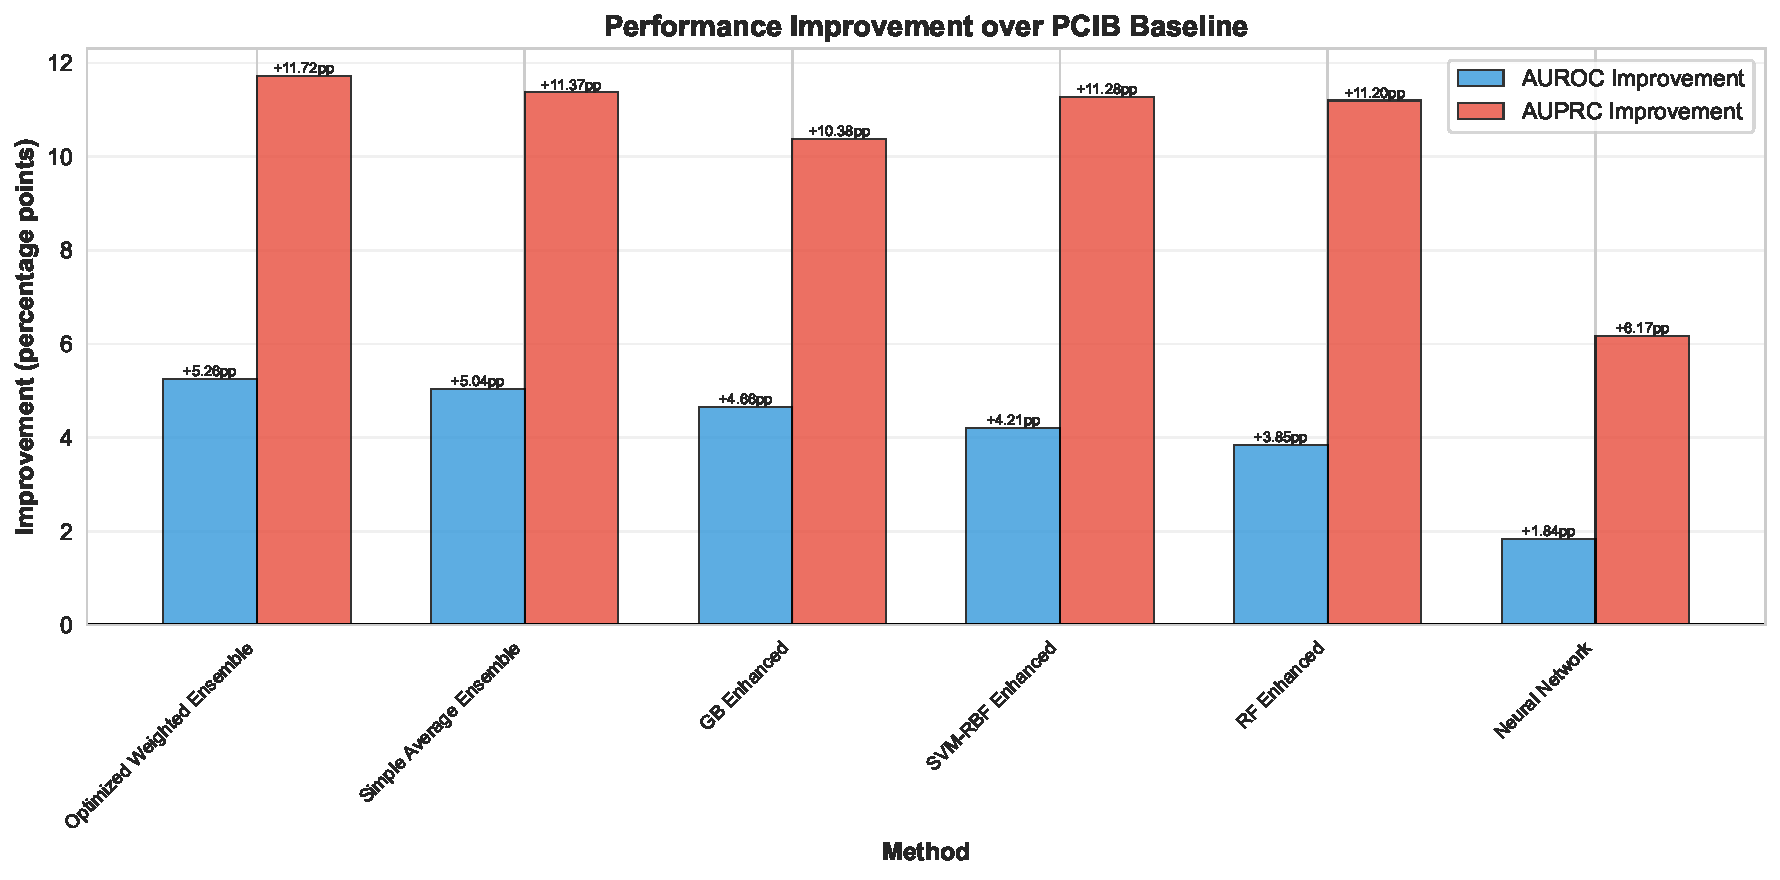
\includegraphics[width=0.9\textwidth]{stacking_improvements.pdf}
  \caption{Improvement over PCIB baseline for each stacking method. Gradient Boosting and ensemble methods provide the largest gains, with improvements of 4-5 percentage points in AUROC. All supervised learning approaches significantly outperform the theory-guided baseline.}
  \label{fig:stacking_improvements}
\end{figure}